\documentclass[11pt,a4paper]{article}
\usepackage[margin=2.3cm]{geometry}
\usepackage{booktabs}
\usepackage{graphicx}
\usepackage{caption}
\usepackage{amsmath}
\usepackage{microtype}
\usepackage[section]{placeins}
\usepackage{xcolor}
\usepackage[colorlinks=true,linkcolor=blue!60!black,urlcolor=blue!60!black]{hyperref}
\captionsetup{font=small,labelfont=bf}
\graphicspath{{plots/}}
\emergencystretch=2em

\newcommand{\UF}{QF\_UF}
\newcommand{\LIA}{QF\_LIA}
\newcommand{\LRA}{QF\_LRA}
\newcommand{\code}[1]{\texttt{#1}}
\newcommand{\nbench}{7,381}
\newcommand{\ncomplete}{7,379}
\newcommand{\nran}{7,159}
\newcommand{\nholes}{2,593,653}
\newcommand{\nattempted}{2,593,653}
\newcommand{\nclosed}{1,036,355}
\newcommand{\closedshare}{40.0}
\newcommand{\ntried}{747,424}
\newcommand{\triedshare}{28.8}
\newcommand{\bridgedshare}{99.24}
\newcommand{\nkept}{1,653}
\newcommand{\workerhours}{216.8}
\newcommand{\passhours}{42.9}
\newcommand{\checkonlyhours}{37.8}
\newcommand{\egglogshare}{78}
\newcommand{\reconshare}{12}
\newcommand{\rwvalid}{4,679}
\newcommand{\dslvalid}{5,245}
\newcommand{\nboth}{4,669}
\newcommand{\dslonly}{576}
\newcommand{\rwonly}{10}


\title{cvc5's rewrite holes, reproved and elaborated by Carcara:\\
  what the pipeline is made of, and what run \code{rw5} costs}
\author{Carcara branch \code{egglog/rewrite-holes} (= \code{egglog/bounded-parallel-holes})}
\date{Run \code{rw5} of 2026-09-27/28 (Carcara \code{7ec65b7d}) and the
  \code{dsl1} arm of 2026-09-25 -- report of 2026-09-29}

\begin{document}
\maketitle

\begin{abstract}
  At \code{--proof-granularity=rewrite}, cvc5 prints one premise-free
  \code{hole} step per call of its rewriter. Carcara reproves each hole with
  a normalizer built from its own checker rules or with egglog saturation
  over RARE rules, reconstructs an Alethe derivation, and splices it in.
  This report describes, briefly, the parts added to that pipeline in the
  last weeks (\S\ref{sec:parts}), and answers four questions from run
  \code{rw5}: \nbench{} benchmarks of \UF{}, \LIA{} and \LRA{}, \nholes{}
  distinct holes in the \nran{} proofs whose elaboration pass finished
  (\S\ref{sec:questions}). \textbf{(1)}~The normalizer closes
  \closedshare\% of the holes at a few milliseconds each and gives egglog a
  normal form for another \triedshare\%; measured on and off before
  \code{rw5}, it is the difference between 71\% and 98\% of the holes
  proved. \textbf{(2)}~A hole egglog proves costs 0.2\,s (\UF{}), 0.5\,s
  (\LRA{}) or 1.2\,s (\LIA{}) of worker time on average. \textbf{(3)}~The
  reconstruction is 11\% of that time and 12\% of the pass; the elaborated
  proofs re-check 25 times faster than they are produced.
  \textbf{(4)}~cvc5's own expansion (\code{dsl-rewrite}) gives \dslvalid{}
  valid proofs against \rwvalid{}, in a seventh of the time.
\end{abstract}

\section{Setting}

Each benchmark runs on half an \code{octa} node (8 cores, 60\,GB):
\begin{enumerate}
  \item cvc5 (branch \code{alethe-rewrite-granularity}) with
    \code{--proof-granularity=rewrite --proof-alethe-res-pivots
    --proof-elim-subtypes --print-arith-lit-token}, 60\,s. Its holes are
    tagged \code{MACRO\_REWRITE} or \code{MACRO\_SR\_PRED\_INTRO}; the
    arithmetic preprocessing and subtype-elimination trust steps are
    attempted too; the theory lemmas (\code{THEORY\_LEMMA}, \code{DIAMONDS})
    never.
  \item Pass 0, \code{carcara elaborate --pipeline hoist prune}, 300\,s
    (\S\ref{sec:hoist}).
  \item Pass 1, \code{carcara elaborate --pipeline hole} with a 92-rule RARE
    file: the normalizer, then the holes on 8 workers, 60\,s and 5.5\,GB per
    hole, 1,500\,s for the pass; the certificates are checked as they are
    spliced in.
  \item \code{carcara check} of the elaborated proof, 1,200\,s.
\end{enumerate}
The comparison arm \code{dsl1} runs the same cvc5 at
\code{--proof-granularity=dsl-rewrite}, where cvc5 expands every rewrite
into RARE rule applications itself, and checks the proof with
\code{carcara check} (900\,s); no egglog.

\section{The pipeline's parts}\label{sec:parts}

\subsection{Before any hole: hoist and prune}\label{sec:hoist}

cvc5 prints a rewrite once for every subproof that uses it. Pass~0
(\code{6364ff71}) checks the proof's steps, computes a digest of every
closed derivation (holes included), lifts each one that repeats to the top
level once and makes its copies references; \code{prune} then drops what
the conclusion no longer reaches. The hoisted proof is printed with term
sharing: printed unshared, a 2.4\,MB proof had become 12\,GB. Within the
pass, holes with the same goal under the same assumptions share one run (the
verdict memo). Table~\ref{tab:hoist}: 4.6\,M hole steps become 2.6\,M
distinct holes, 2.3--2.4 times fewer on the arithmetic logics, in 3.1\,h
summed; 206 proofs are rejected before any hole by cvc5's resolution-pivot
defect.

\begin{table}[htbp]
  \centering\small
  \resizebox{\textwidth}{!}{\begin{tabular}{lrrrr}
\toprule
 & \UF{} & \LIA{} & \LRA{} & all \\
\midrule
proofs (complete in 60\,s) & 4,316 & 2,539 & 524 & 7,379 \\
\quad hoisted & 4,118 & 2,529 & 518 & 7,165 \\
\quad rejected upfront (cvc5's resolution pivots) & 198 & 2 & 6 & 206 \\
\quad hoist out of time (300\,s) & 0 & 8 & 0 & 8 \\
\midrule
hoisted proofs: hole steps printed by cvc5 & 1,239,039 & 2,132,077 & 1,261,973 & 4,633,089 \\
\quad distinct holes after hoist and prune & 1,171,831 & 915,032 & 522,311 & 2,609,174 \\
\quad ratio & 1.06 & 2.33 & 2.42 & 1.78 \\
\quad proofs with fewer holes after it & 2,271 & 1,231 & 386 & 3,888 \\
\quad commands pruned, of all & 0.3\% & 20.5\% & 1.1\% & 2.7\% \\
\quad time, median / max & 363\,ms / 169.7\,s & 14\,ms / 238.3\,s & 74\,ms / 20.0\,s & 168\,ms / 238.3\,s \\
\quad time, summed (h) & 1.3 & 1.6 & 0.1 & 3.1 \\
\bottomrule
\end{tabular}
}
  \caption{Pass 0 on the proofs cvc5 completed in 60\,s.}
  \label{tab:hoist}
\end{table}

\subsection{The pre-normalizer}\label{sec:prenorm}

\code{--hole-prenormalize} (\code{src/elaborator/prenorm.rs}). Before any
hole is scheduled, both sides of every hole are normalized bottom-up, with
one memo per proof, by five of the checker's own procedures:
\code{evaluate} on ground terms; \code{poly\_simp}, arithmetic to the
checker's canonical polynomial; \code{poly\_simp\_rel}, a relation to
\code{(op P c)} with the difference scaled to integral coefficients of gcd~1
(Int) or leading coefficient~1 (Real), equalities oriented; \code{aci\_simp},
\code{and}/\code{or} flattened, identities dropped, duplicates removed,
arguments sorted; \code{distinct\_elim}; and one fold, two mirrored bounds
among a conjunction's arguments to their equality (\code{la\_rw\_eq}). Every
step is one rule applied to one subterm, so a normal form comes with its
certificate (\code{cong}, \code{trans}, \code{symm} around those steps).
When the two sides meet, that certificate replaces the hole and egglog never
runs. Otherwise egglog gets the equality of the normal forms first, on a
third of the hole's budget, and its certificate is bridged back to the stated
sides by the normalizer's derivations; if that fails, the goal as stated
gets the whole budget. The normalizer stays within core Alethe: Boolean
simplification, relation flips and integer tightening are RARE rules, and
egglog's job. Its orders are term pointers, canonical within a run but not
between runs, which is where \code{rw5}'s run-to-run differences on
\code{rings} came from.

\subsection{The set encoding of \code{and}/\code{or}}\label{sec:setform}

egglog stores a term's arguments as a chain, and a RARE rule with $k$
\code{:list} parameters has to bind segments of it: the \code{chain}
encoding does that by re-association and $2^k-1$ variants of the rule for
the empty lists. \code{--rare-list-encoding set-form} (the default) also
represents every \code{and}/\code{or} as the set of its arguments, with
rules for identity and absorbing elements, and compiles a rule whose
left-hand side is an \code{and}/\code{or} over \code{:list} parameters
\emph{once} on that form, its fixed arguments becoming membership
conditions: it fires at any arity, in any position, with empty lists. The
set forms of derived terms come from a ruleset of their own that runs only
as egglog's last fallback, so a goal the ordinary rules prove pays nothing
for them; since \code{rw5}, membership is a relation filled by position and
splicing a nested \code{and}/\code{or} into its parent is guarded. Measured
before: on veriT's Boolean-heavy holes the set form proves 83\% more holes in
the same budget (98 proofs). On cvc5's holes the two encodings are a wash:
over the whole corpus at theory-rewrite granularity (\code{enc4}) they prove
70.7\% and 70.6\% of the holes without the normalizer and 98.3\% each with
it, in 112\,h and 113\,h, and 50\,h each.

\subsection{Sort guards}\label{sec:guards}

egglog's rules range over one untyped sort of terms, so an arithmetic rule
matched Boolean and uninterpreted terms: \code{arith-eq-elim} fired 12,000
times on \UF{} goals. \code{--rare-sort-guards} (\code{58bc6945}) keeps
relations \code{SortInt}, \code{SortReal}, \code{SortBool} (later
\code{String}, \code{RegLan}) on e-classes, seeded from the goal's subterms
by their declared sorts and propagated by operator (Bool for connectives
and comparisons, Real for \code{/} and \code{to\_real}, the argument's sort
for \code{+ - *}, the branch's for \code{ite}, the declared result for an
uninterpreted function), and adds a guard premise for every Int, Real or
Bool parameter of a rule. The certificate search strips the guards, so the
certificates do not change. On the ten sample proofs of the time the kept
holes went from 267 to 169 with the ACI identity rules of the same day, and
to 129 with the guards; micro-goals ran 2 to 4 times faster.

\subsection{Premise seeding}\label{sec:seeding}

A conditional RARE rule fires only when its premise holds in the e-graph,
so the premise's terms must exist, and the rule compiler adds a
\emph{demand} rule that builds them. The first demand built every premise
over all pairs of available terms, whatever their sorts: on a \UF{} goal of
twelve conjuncts, eight such rules fired 2,175 times each in the second round
and 12,775 in the fourth, and \code{eq-cond-deq} matched 530,000 times in
one round; a 28-conjunct hole of the corpus died at 6\,GB, where its proof
had checked in under a second at theory-rewrite granularity. Two designs were measured. Seeding the premises
from the goal's subterms only (\code{--rare-seed-from-goal},
\code{29e4f7f3}) was 5\% faster and lost 9 provable holes of the sample, so
it is not used. \emph{Demand at the left-hand side} (\code{d78da84d}, with
\code{6fa30dbf}) builds a premise's terms exactly for the bindings of each
occurrence of the rule's left-hand side, where the rule could fire; a
premise variable the left-hand side does not bind ranges over the seed
relation under its sort guard, and no all-pairs seeding is left. Such
goals then take 0.2--0.3\,s at every size up to 28 conjuncts; on the ten
samples every hole but two is proved and the passes run 1.3 to 10 times
faster; on 23 local proofs the unproved holes went from 56 to 6 and the pass
from 903\,s to 475\,s. \code{rw2}, the first run with it (and with a
larger pass budget), checked 99.9/99.7/99.5\% of the holes
(\UF{}/\LIA{}/\LRA{}) against \code{rw1}'s 99.6/95.8/85.7\%.

\subsection{The parallel setup}\label{sec:parallel}

\begin{itemize}
  \item \textbf{A process per hole} (\code{--hole-isolate}), eight at a
    time (\code{--hole-threads 8}), under a hard time limit (the child is
    killed at 60\,s) and an address-space limit of 5.5\,GB, the job's 60\,GB
    less 16\,GB for the driver over eight, with a soft cap at 90\% for a
    clean stop. A killed or failed child leaves its hole as a trusted hole
    with a reason class, and the rest of the proof goes on. A process is
    the only hard bound: an egglog iteration cannot be interrupted, and in
    one process a 1\,s budget was overrun sixty-fold.
  \item \textbf{A process per attempt.} Within a hole every attempt runs in
    a fresh process with its share of the hole's budget: the normalized
    goal (a third), the abstract goal (shared subterms of 16 nodes or more
    as constants; half), the whole goal (a quarter, at most 10\,s), the
    structural descent over atom pairs (at least 8\,s a pair), the atom
    alignment, the whole goal again. Each is killed 3\,s past its share and
    dies with its parent. A process that had failed once was where every
    later attempt met the memory limit.
  \item \textbf{A pass budget} of 1,500\,s from Carcara's start: holes not
    started when it runs out are kept, and the pass ends with its partial
    result. Holes are scheduled smallest goal first, so a binding budget
    covers the most holes (12 to 75 times more on three \LRA{} proofs).
  \item \textbf{Text across the boundary.} A child returns the certificate
    as text, which the parent parses, checks and splices into the proof,
    one hole at a time.
  \item \textbf{A runner whose records survive a kill:} each pass's keys are
    printed as soon as they are known, and the kept holes are counted by
    class.
\end{itemize}
In \code{rw5} (Table~\ref{tab:pass}) the workers are busy 73\% of the hole
phase (\UF{} 56\%: small proofs and the tails of large ones), starting a
process and parsing its input costs 25\,ms a hole (10\% of the worker time),
no task used more than 37.8\,GB of its 60\,GB, the pass budget cut 36
holes, and every task kept its record. 14 passes (Dartagnan and
\code{nec-smt} proofs) were killed at the external limit of 1,600\,s and
count as unfinished.

\section{Four questions}\label{sec:questions}

\subsection{With the normalizer, or without?}\label{sec:q-norm}

\code{rw5} ran with the normalizer, so its effect is read within the run
(Table~\ref{tab:norm}) and from two earlier on/off measurements
(Table~\ref{tab:onoff}).

\textbf{Within \code{rw5}.} The normalizer closes \nclosed{} holes,
\closedshare\% (\UF{} 13\%, \LIA{} 61\%, \LRA{} 64\%), for 466\,s of
normalization and 0.75\,h of certificate checking in all: 3\,ms a hole,
against 0.2 to 1.2\,s for a hole egglog proves. It gives egglog a normal
form for another \triedshare\% of the holes, and \bridgedshare\% of those are
proved and bridged; of the 5,660 that are not, 3,997 are proved as stated.
The normal forms are smaller than the goals for 86\% of the \UF{} ones and
larger for 52\% of \LIA{}'s (the polynomial form with its \code{(* -1 x)}
monomials). The remaining 31\% of the holes are goals the normalizer leaves
unchanged, and none of the \nkept{} kept holes is among them: every kept hole
had been given a normal form first. Sent to egglog instead, the closed holes
would cost at least the floor of a worker hole (the cheapest 1\% cost
0.15\,s in \UF{}, 0.16\,s in \LIA{}, 0.21\,s in \LRA{}): about 50\,h of worker
time more, nearly a quarter on top of the run's \workerhours\,h.

\begin{table}[htbp]
  \centering\small
  \resizebox{\textwidth}{!}{\begin{tabular}{lrrrr}
\toprule
 & \UF{} & \LIA{} & \LRA{} & all \\
\midrule
holes (proofs whose pass finished) & 1,171,831 & 899,511 & 522,311 & 2,593,653 \\
closed by the normalizer & 155,455 (13.3\%) & 549,155 (61.1\%) & 331,745 (63.5\%) & 1,036,355 (40.0\%) \\
normal form tried first & 340,595 (29.1\%) & 245,973 (27.3\%) & 160,856 (30.8\%) & 747,424 (28.8\%) \\
\quad proved and bridged & 339,758 (99.75\%) & 241,402 (98.14\%) & 160,604 (99.84\%) & 741,764 (99.24\%) \\
\quad not, retried as stated: proved & 292 of 837 & 3,583 of 4,571 & 122 of 252 & 3,997 of 5,660 \\
\quad normal form smaller / same / larger (\%) & 86 / 14 / 0 & 25 / 23 / 52 & 18 / 53 / 29 & 51 / 25 / 24 \\
goal unchanged by the normalizer & 675,781 (57.7\%) & 104,383 (11.6\%) & 29,710 (5.7\%) & 809,874 (31.2\%) \\
\midrule
normalization and closing certificates (s) & 52.1 & 224.6 & 189.3 & 466.0 \\
inserting the closed holes' certificates (s) & 28.7 & 1,725.7 & 944.2 & 2,698.5 \\
worker time of the other justified holes (h) & 60.2 & 112.2 & 26.9 & 199.3 \\
\bottomrule
\end{tabular}
}
  \caption{The normalizer in the elaboration pass. ``Normal form tried
    first'': egglog on the equality of the normal forms, on a third of the
    hole's budget; ``bridged'': its certificate connected to the stated sides
    by the normalizer's derivations. Normalization time includes building
    the closing certificates.}
  \label{tab:norm}
\end{table}

\textbf{Before \code{rw5}}, measured on and off: over the whole corpus at
theory-rewrite granularity (run \code{enc4}, checking only, 5.44\,M holes)
the normalizer took the proved holes from 70.7\% to 98.3\% and the passes
from 112\,h to 50\,h; at rewrite granularity on ten sample proofs, from
85.2\% to 99.7\% of the holes and from 2 to 6 fully proved proofs, in a
quarter of the time. A rewrite-granularity hole is one call of the whole
rewriter on a term, and without the normalizer egglog pays for its size.

\begin{table}[htbp]
  \centering\small
  \resizebox{\textwidth}{!}{%
  \begin{tabular}{llrrrrr}
    \toprule
    & & holes & proved & closed by the normalizer & proofs fully proved & pass time \\
    \midrule
    \code{enc4}: theory-rewrite, & without & 5,441,531 & 70.7\% & -- & 3,523 & 112\,h \\
    \quad 7,192 proofs (2026-09-20) & with & 5,440,377 & 98.3\% & 57.5\% & 6,775 & 50\,h \\
    \midrule
    rewrite, ten sample & without & 7,889 & 85.2\% & -- & 2 & 2,094\,s \\
    \quad proofs (2026-09-22) & with & 7,889 & 99.7\% & 38.4\% & 6 & 547\,s \\
    \bottomrule
  \end{tabular}}
  \caption{The normalizer on and off, checking only, before \code{rw5}
    (notes \S36 and \S47.2; 60\,s and 8\,GB per hole and 600\,s per proof,
    respectively 30\,s, 3.5\,GB and 300\,s). In \code{enc4} most of the
    difference is holes never attempted within the proof's budget (1.56\,M
    without, 76,000 with).}
  \label{tab:onoff}
\end{table}

\subsection{The cost of a hole}\label{sec:q-cost}

A hole's cost is its worker time: the wall time of its processes, every
attempt included (Table~\ref{tab:cost}, Figure~\ref{fig:cost}). In \UF{} a
hole egglog proves costs 0.21\,s on average and hardly any deviates (p99
0.33\,s): the fixed cost of a fresh process, the rule program and a short
saturation, of which about 0.15\,s is the floor. \LIA{}'s cost 1.2\,s on
average (median 0.75\,s, p99 10\,s; the tail is Dartagnan's whole-assertion
holes) and \LRA{}'s 0.51\,s (median 0.27\,s). A kept hole costs what its
limits let it spend, 28 to 48\,s on average and 17\,h in all (8\% of the
worker time). Over all holes, closed ones included, a hole costs 0.20\,s
(\UF{}, \LRA{}) or 0.50\,s (\LIA{}); the \nholes{} holes take \workerhours\,h
of worker time in \passhours\,h of pass time, a median pass of 7.6\,s a
proof (Table~\ref{tab:pass}).

\begin{table}[htbp]
  \centering\small
  \resizebox{\textwidth}{!}{\begin{tabular}{llrrrrrrrr}
\toprule
 & holes & number & \% & mean & median & p90 & p99 & max & hours \\
\midrule
\UF{} & closed by the normalizer & 155,455 & 13.27 & 0.5\,ms & 0.3\,ms & 0.3\,ms & 3.3\,ms & 49\,ms & 0.0 \\
 & justified through egglog & 1,015,831 & 86.69 & 213\,ms & 222\,ms & 228\,ms & 326\,ms & 47.0\,s & 60.2 \\
 & kept & 545 & 0.05 & 27.8\,s & 30.0\,s & 30.2\,s & 60.2\,s & 60.2\,s & 4.2 \\
 & all & 1,171,831 & 100.00 & 198\,ms & 215\,ms & 227\,ms & 316\,ms & 60.2\,s & 64.4 \\
\midrule
\LIA{} & closed by the normalizer & 549,155 & 61.05 & 3.6\,ms & 2.4\,ms & 6.4\,ms & 21\,ms & 375\,ms & 0.5 \\
 & justified through egglog & 349,365 & 38.84 & 1.2\,s & 750\,ms & 1.3\,s & 10.1\,s & 79.9\,s & 112.2 \\
 & kept & 978 & 0.11 & 42.3\,s & 60.0\,s & 62.6\,s & 72.9\,s & 75.3\,s & 11.5 \\
 & all & 899,498 & 100.00 & 497\,ms & 3.4\,ms & 944\,ms & 5.2\,s & 79.9\,s & 124.2 \\
\midrule
\LRA{} & closed by the normalizer & 331,745 & 63.51 & 3.4\,ms & 1.6\,ms & 5.6\,ms & 23\,ms & 2.1\,s & 0.3 \\
 & justified through egglog & 190,436 & 36.46 & 509\,ms & 270\,ms & 892\,ms & 1.8\,s & 62.4\,s & 26.9 \\
 & kept & 130 & 0.02 & 48.1\,s & 60.0\,s & 60.2\,s & 70.6\,s & 74.2\,s & 1.7 \\
 & all & 522,311 & 100.00 & 200\,ms & 3.6\,ms & 645\,ms & 1.5\,s & 74.2\,s & 29.0 \\
\bottomrule
\end{tabular}
}
  \caption{Cost per hole. For a hole egglog proves or that is kept, the
    worker time; for a hole the normalizer closes, its share of the proof's
    normalization plus the check of its certificate in the parent. A kept
    hole's time is its last attempt's kill time or its phases, whichever is
    larger.}
  \label{tab:cost}
\end{table}

\begin{figure}[htbp]
  \centering
  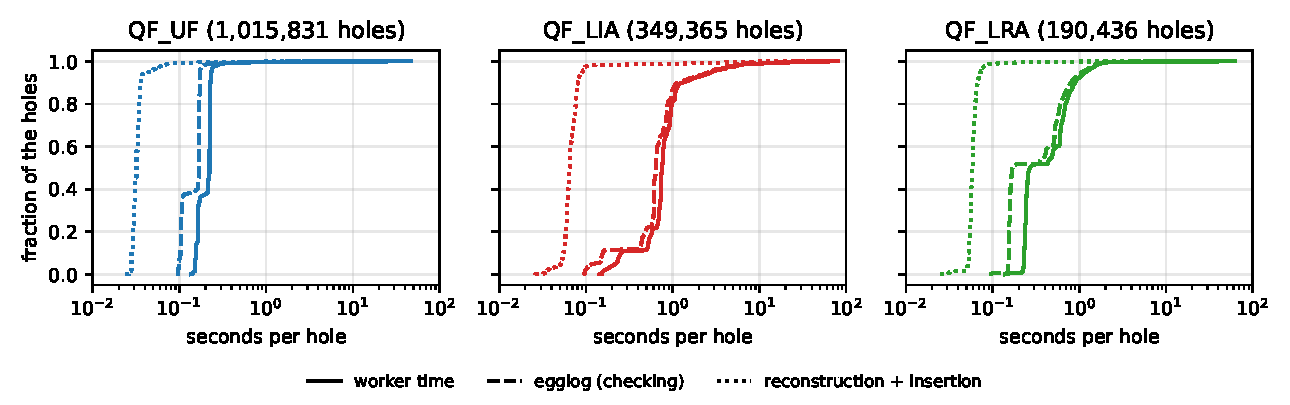
\includegraphics[width=\textwidth]{hole-cost}
  \caption{The holes egglog proved: worker time per hole, its egglog
    phases (what a checking-only pass runs), and its reconstruction phases
    with the insertion (what elaboration adds). The steps are the
    per-logic floors: a process, the rule program, the first rounds.}
  \label{fig:cost}
\end{figure}

\subsection{Elaboration against checking}\label{sec:q-elab}

\textbf{Per hole the split is exact} (Table~\ref{tab:phases}). For the
1.56\,M holes justified through egglog, the saturation that decides the goal,
which is what a checking-only pass runs, is \egglogshare\% of the worker time;
reconstructing the certificate from the saturated e-graph is 11\%, nearly
all of it the certificate search; inserting and checking its steps 1\%;
starting the process 10\%. The median hole spends 168\,ms in egglog and
34\,ms in reconstruction and insertion, and for 0.2\% of the holes the
reconstruction costs more than egglog. What the reconstruction loses costs
more: 868 holes were kept in the reconstruction after egglog had proved their
goal or a descent pair of it (killed in one of its phases, no certificate,
or the certificate rejected), 12\,h of worker time.

\textbf{Per proof it is an estimate}: the pass less its holes'
reconstruction phases spread over the eight workers and less the insertion
comes to \checkonlyhours\,h for a checking-only pass, against \passhours\,h
for elaboration, which therefore adds 12\% (Table~\ref{tab:pass}). The
result is cheap to check: the 6,585 proofs with every hole justified
re-check in 1.0\,h in all (median 0.14\,s), against the 25.3\,h their
elaboration took, with twice the steps of the hoisted proof.

\begin{table}[htbp]
  \centering\small
  \resizebox{\textwidth}{!}{\begin{tabular}{lrrrr}
\toprule
justified holes through egglog, hours & \UF{} & \LIA{} & \LRA{} & all \\
\midrule
egglog: saturation, the goal decided & 42.3 (70\%) & 92.0 (81\%) & 22.0 (81\%) & 156.3 (78\%) \\
reconstruction & 10.0 (16\%) & 9.8 (9\%) & 3.1 (12\%) & 22.9 (11\%) \\
\quad serializing the e-graph & 0.4 (1\%) & 0.7 (1\%) & 0.2 (1\%) & 1.3 (1\%) \\
\quad indexing it & 0.0 (0\%) & 0.1 (0\%) & 0.0 (0\%) & 0.2 (0\%) \\
\quad searching for the certificate & 9.5 (16\%) & 8.7 (8\%) & 3.0 (11\%) & 21.2 (11\%) \\
\quad emitting the steps & 0.0 (0\%) & 0.3 (0\%) & 0.0 (0\%) & 0.3 (0\%) \\
inserting and checking the steps & 0.2 (0\%) & 0.9 (1\%) & 0.1 (0\%) & 1.3 (1\%) \\
process start and input parsing & 7.9 (13\%) & 10.4 (9\%) & 1.8 (7\%) & 20.1 (10\%) \\
\midrule
per hole, median: egglog / elaboration & 167\,ms / 32\,ms & 644\,ms / 64\,ms & 170\,ms / 58\,ms & 168\,ms / 34\,ms \\
holes whose elaboration costs more than egglog (\%) & 0.0 & 0.4 & 0.2 & 0.2 \\
\midrule
kept after egglog proved the goal: holes, worker time & 266, 2.3\,h & 488, 8.1\,h & 114, 1.6\,h & 868, 12.1\,h \\
\bottomrule
\end{tabular}
}
  \caption{Worker time of the holes egglog proved and the reconstruction
    justified, by phase. ``Elaboration'' per hole: reconstruction and
    insertion. The last row is the kept holes that egglog had proved.}
  \label{tab:phases}
\end{table}

\begin{table}[htbp]
  \centering\small
  \resizebox{\textwidth}{!}{\begin{tabular}{lrrrr}
\toprule
 & \UF{} & \LIA{} & \LRA{} & all \\
\midrule
proofs whose pass finished & 4,118 & 2,523 & 518 & 7,159 \\
elaboration pass (h) & 15.9 & 21.4 & 5.6 & 42.9 \\
\quad normalizer & 0.0 & 0.1 & 0.1 & 0.1 \\
\quad holes in the workers & 14.5 & 17.8 & 5.0 & 37.3 \\
\quad inserting and checking the certificates & 0.2 & 1.4 & 0.4 & 2.0 \\
\quad the rest: parsing, the other steps, printing & 1.2 & 2.1 & 0.2 & 3.5 \\
checking-only pass, estimated (h) & 14.4 & 18.6 & 4.8 & 37.8 \\
\quad elaboration's share of the pass (\%) & 9.5 & 12.9 & 13.9 & 11.8 \\
worker time (h) & 64.4 & 123.7 & 28.7 & 216.8 \\
\quad utilization of the 8 workers (\%) & 55.6 & 86.8 & 72.2 & 72.7 \\
pass time per proof, median / p90 & 9.2\,s / 37.1\,s & 1.5\,s / 66.4\,s & 4.6\,s / 125.8\,s & 7.6\,s / 54.9\,s \\
task memory, p99 / max (GB) & 3.5 / 7.9 & 15.4 / 37.8 & 6.1 / 9.1 & 6.1 / 37.8 \\
\midrule
proofs with every hole justified, re-checked & 3,718 & 2,420 & 447 & 6,585 \\
\quad elaboration pass, median / sum & 8.6\,s / 9.7\,h & 1.3\,s / 12.8\,h & 2.3\,s / 2.8\,h & 6.8\,s / 25.3\,h \\
\quad re-check of the elaborated proof, median / sum & 272\,ms / 0.6\,h & 15\,ms / 0.3\,h & 52\,ms / 0.1\,h & 138\,ms / 1.0\,h \\
\quad steps: hoisted proof / elaborated, median & 27,134 / 32,125 & 126 / 520 & 468 / 4,138 & 6,254 / 12,551 \\
\bottomrule
\end{tabular}
}
  \caption{The elaboration pass per proof. ``Holes in the workers'' is the
    wall time of the hole phase; the worker time is what the eight workers
    spent in it. The checking-only pass is estimated, as described in the
    text.}
  \label{tab:pass}
\end{table}

\subsection{Against cvc5's own expansion}\label{sec:q-cvc5}

Table~\ref{tab:cvc5}, Figures~\ref{fig:cvc5}--\ref{fig:scatter}. Three
routes lead from a benchmark to a proof checked in full.
\emph{cvc5-dsl + check}: cvc5 at \code{dsl-rewrite} and \code{carcara check},
the proof re-checked \code{valid} (\code{dsl1}). \emph{cvc5-rw + check}: cvc5
at \code{rewrite}, the hoist, and a checking-only pass, every hole checked
and no untagged hole left; its time is the estimate of
\S\ref{sec:q-elab}. \emph{cvc5-rw + check + elab}: cvc5 at \code{rewrite},
the hoist, the elaboration pass and the re-check, the proof re-checked
\code{valid} (\code{rw5}). Figure~\ref{fig:cvc5} draws them with the
fraction of the benchmarks on the $y$ axis, Figure~\ref{fig:cvc5-count}
with their number.

\textbf{Producing.} At \code{dsl-rewrite} cvc5 takes 15\% more time
(6.1\,h against 5.3\,h summed, median 0.68\,s against 0.53\,s), loses 22
proofs to its 60\,s limit, and prints 7\% more text. Its expansion of every
rewrite thus costs it about 0.8\,h, around a millisecond a hole, against
0.3\,s of worker time a hole in Carcara.

\textbf{Outcome.} The three routes check \dslvalid{}, \checkfull{} and
\rwvalid{} proofs in full. With elaboration, \nboth{} are checked by both
cvc5-dsl and the rewrite route, \rwonly{} only by the rewrite route, and
\dslonly{} only by cvc5-dsl, 567 of which have a hole \code{rw5} kept or did
not reach; with checking only, \checkdslonly{} are left to cvc5-dsl alone.
In \UF{} all three are capped by the \code{THEORY\_LEMMA} holes of 1,789
proofs, which none of them attempts.

\textbf{Time.} On the \nboth{} proofs valid in both, a checked proof takes
5.2\,s with \code{rw5} against 0.42\,s with \code{dsl1} (median), 22.5\,h
against 3.1\,h summed. Checking only does not close the gap: the two
rewrite routes nearly coincide in Figure~\ref{fig:cvc5}, the cost being
egglog's, not the reconstruction's. Per benchmark (Figure~\ref{fig:scatter}a
and~b) the rewrite routes lie above the diagonal almost everywhere; they
are faster on \elabfaster{} of the \nboth{} benchmarks checked with
elaboration and on \checkfaster{} of the \checkboth{} checked without, and
those are tiny proofs (345 of the \elabfaster{} from SMPT) on which every
route takes a few tens of milliseconds.

\textbf{The proofs.} \code{rw5}'s elaborated proofs have 1.4 times
\code{dsl1}'s steps (98.5\,M against 68.9\,M; 3.2\,M \code{rare\_rewrite}
steps against 2.4\,M, fewer in \LRA{}, where the normalizer's
\code{poly\_simp} and \code{aci\_simp} steps stand in) and are checked in
the same time (0.5\,h each, medians 69 and 58\,ms). Per proof
(Figure~\ref{fig:scatter}c and~d) the elaborated proof is larger on all but
\stepsbelow{} of the \nboth{} (median \stepsratio{} times), and its check
takes \checkratio{} times cvc5's at the median, within 0.70 to 1.55 times
on 80\% of the proofs, and is faster on \checkbelow{} of them.

\begin{table}[htbp]
  \centering\small
  \resizebox{\textwidth}{!}{\begin{tabular}{lrrrr}
\toprule
 & \UF{} & \LIA{} & \LRA{} & all \\
\midrule
benchmarks & 4,316 & 2,541 & 524 & 7,381 \\
complete proof in 60\,s: rewrite / dsl-rewrite & 4,316 / 4,316 & 2,539 / 2,531 & 524 / 510 & 7,379 / 7,357 \\
cvc5 time, median: rewrite / dsl-rewrite & 810\,ms / 982\,ms & 48\,ms / 88\,ms & 198\,ms / 388\,ms & 526\,ms / 681\,ms \\
cvc5 time, summed (h): rewrite / dsl-rewrite & 3.1 / 3.4 & 1.4 / 1.8 & 0.8 / 1.0 & 5.3 / 6.1 \\
proof text (GB): rewrite / dsl-rewrite & 22.0 / 22.3 & 3.2 / 4.2 & 1.4 / 2.1 & 26.7 / 28.6 \\
\midrule
re-checked \code{valid}: rw5 / dsl1 & 1,828 / 2,230 & 2,404 / 2,510 & 447 / 505 & 4,679 / 5,245 \\
\quad both / rw5 only / dsl1 only & 1,828 / 0 / 402 & 2,402 / 2 / 108 & 439 / 8 / 66 & 4,669 / 10 / 576 \\
checked in full: cvc5-dsl + check / cvc5-rw + check / + elab & 2,230 / 1,975 / 1,828 & 2,510 / 2,438 / 2,404 & 505 / 469 / 447 & 5,245 / 4,882 / 4,679 \\
valid in both, time to a checked proof, median: rw5 / dsl1 & 6.8\,s / 617\,ms & 1.6\,s / 90\,ms & 2.4\,s / 185\,ms & 5.2\,s / 415\,ms \\
\quad summed (h): rw5 / dsl1 & 5.0 / 0.7 & 14.3 / 1.6 & 3.2 / 0.8 & 22.5 / 3.1 \\
\quad final proof's check, median: rw5 / dsl1 & 124\,ms / 95\,ms & 15\,ms / 16\,ms & 50\,ms / 29\,ms & 69\,ms / 58\,ms \\
\quad final proof's check, summed (h): rw5 / dsl1 & 0.1 / 0.1 & 0.3 / 0.3 & 0.1 / 0.1 & 0.5 / 0.5 \\
\quad steps, median: rw5 elaborated / dsl1 & 12,365 / 9,475 & 502 / 274 & 3,889 / 1,144 & 3,918 / 2,372 \\
\quad steps, summed (M): rw5 elaborated / dsl1 & 37.7 / 33.2 & 40.6 / 24.4 & 20.3 / 11.3 & 98.5 / 68.9 \\
\quad \code{rare\_rewrite} steps, summed (M): rw5 / dsl1 & 1.53 / 0.62 & 1.54 / 1.21 & 0.17 / 0.60 & 3.24 / 2.42 \\
\bottomrule
\end{tabular}
}
  \caption{\code{rw5} against \code{dsl1}, the same benchmarks and cvc5;
    cvc5 rows over the proofs complete at both granularities. ``Checked in
    full'': the three routes of the text. A checked proof's time: cvc5,
    hoist, elaboration and re-check for \code{rw5}; cvc5 and check for
    \code{dsl1}.}
  \label{tab:cvc5}
\end{table}

\begin{figure}[htbp]
  \centering
  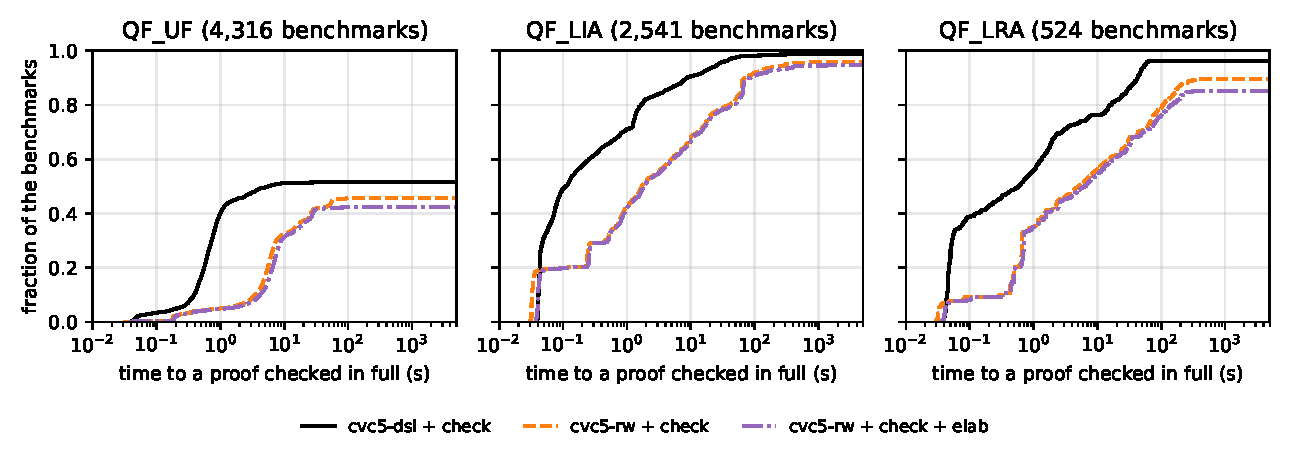
\includegraphics[width=\textwidth]{vs-cvc5}
  \caption{Time from benchmark to a proof checked in full, over every
    benchmark of each logic; a route's line ends at the share of the
    benchmarks it checks in full. \emph{cvc5-dsl + check}: cvc5 at
    \code{dsl-rewrite} and \code{carcara check} (\code{dsl1}).
    \emph{cvc5-rw + check}: cvc5 at \code{rewrite}, hoist and checking-only
    pass (estimated), every hole checked. \emph{cvc5-rw + check + elab}:
    cvc5 at \code{rewrite}, hoist, elaboration pass and re-check
    (\code{rw5}).}
  \label{fig:cvc5}
\end{figure}

\begin{figure}[htbp]
  \centering
  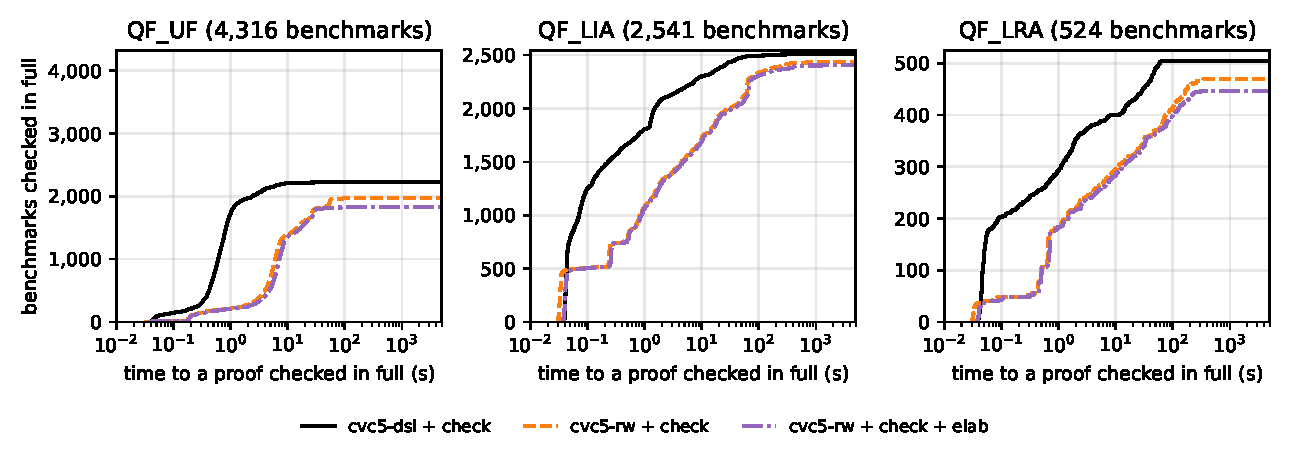
\includegraphics[width=\textwidth]{vs-cvc5-count}
  \caption{Figure~\ref{fig:cvc5} with the number of benchmarks on the $y$
    axis, each panel up to its logic's number of benchmarks.}
  \label{fig:cvc5-count}
\end{figure}

\begin{figure}[htbp]
  \centering
  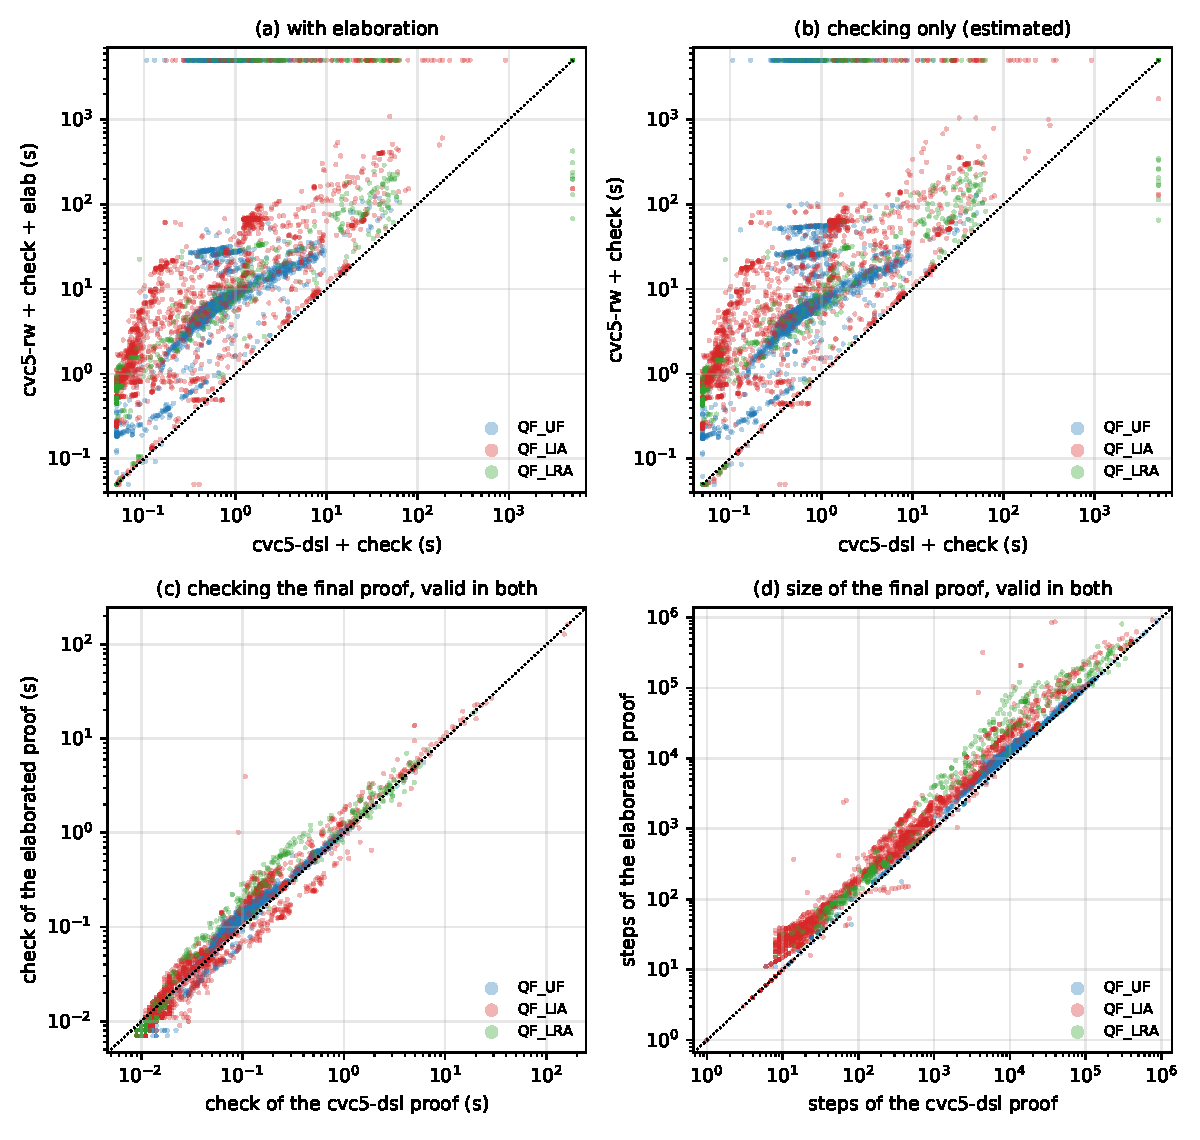
\includegraphics[width=.92\textwidth]{vs-cvc5-scatter}
  \caption{Per benchmark. (a), (b): cvc5-dsl + check ($x$) against
    cvc5-rw + check + elab and cvc5-rw + check ($y$), every benchmark; one a
    route does not check in full sits on that route's edge, one neither
    route checks in the corner. (c), (d): the \nboth{} benchmarks valid in
    both, the check of the final proof and its number of steps, cvc5's own
    expansion ($x$) against the elaborated proof ($y$). The dotted line is
    $y = x$.}
  \label{fig:scatter}
\end{figure}

\section{In short}

\begin{enumerate}
  \item \textbf{Normalizer:} closes \closedshare\% of the holes at 3\,ms each
    and bridges \bridgedshare\% of the normal forms it hands egglog; every
    kept hole is among the goals it changed. Measured on and off, it is
    71\% against 98\% of the holes proved (whole corpus, theory-rewrite) and
    85\% against 99.7\% (ten proofs, rewrite), in half to a quarter of the
    time.
  \item \textbf{Cost of a hole:} 0.20\,s of worker time in \UF{} and \LRA{},
    0.50\,s in \LIA{}, closed holes included; a hole egglog proves has a
    floor of about 0.15\,s, the process and the rule program.
  \item \textbf{Elaboration against checking:} 11\% of the worker time of a
    justified hole, 12\% of the pass; its losses are 868 holes and 12\,h.
    The elaborated proof re-checks 25 times faster than it is produced.
  \item \textbf{Against cvc5:} its own expansion costs it about a
    millisecond a hole against Carcara's 0.3\,s. cvc5-dsl + check,
    cvc5-rw + check and cvc5-rw + check + elab check \dslvalid{}, \checkfull{}
    and \rwvalid{} proofs in full; on the proofs both check, cvc5's route
    takes a seventh of the time. The proofs \code{rw5} elaborates are 1.4
    times larger and check as fast.
\end{enumerate}

\end{document}
